\documentclass[11pt]{article}
\usepackage[letterpaper,margin=2.2cm]{geometry}
\usepackage{booktabs}
\usepackage{enumitem}
\usepackage{titlesec}
\usepackage{xcolor}
\usepackage{microtype}
\usepackage{amsmath}
\usepackage{tikz}
\usetikzlibrary{positioning,calc}
\usepackage[hidelinks]{hyperref}

\titleformat{\section}{\large\bfseries}{\thesection}{0.6em}{}
\titlespacing*{\section}{0pt}{1.2em}{0.5em}
\setlist{nosep, leftmargin=1.4em}
\setlength{\parskip}{0.4em}
\setlength{\parindent}{0pt}

\newcommand{\code}[1]{\texttt{#1}}

\tikzset{
  blk/.style={draw, rounded corners=2pt, minimum height=9mm, minimum width=15mm, align=center, font=\small},
  ina/.style={draw, thick, fill=gray!20, minimum height=9mm, minimum width=13mm, align=center, font=\small},
  pw/.style={very thick},
  dat/.style={densely dashed},
  lbl/.style={font=\scriptsize, text=black!70},
}

\begin{document}

{\centering
{\LARGE\bfseries Power Measurement Wiring}\\[0.4em]
{\large One board at a time, at its 5\,V input, nothing cut}\\[0.3em]
{\small 2 November 2026, revision 3: one spare F411 as USB breakout and logger; the Pi by its own telemetry}\par}

\section{The plan}

We have six INA226 current-sense modules. Each one has a small resistor, the \emph{shunt},
that the measured current flows through; the chip reads the voltage across it and the supply
voltage, and reports both over I$^2$C to a logger.

\begin{itemize}
\item \textbf{One board at a time.} Only the board under test is connected. Then everything is
unplugged and the next board is wired up.
\item \textbf{One module per board, in its 5\,V supply wire.} Nothing on any board is cut,
lifted or soldered. On the three microcontroller boards the module sits between the spare
F411, used as a USB breakout, and one of our USB-A female breakouts. The Pi is not wired at
all: it reports its own power (section~5).
\item \textbf{One address.} With one module on the bus at a time, every module stays at the
breakout's default address, \code{0x40} (\code{A0} and \code{A1} to ground).
\end{itemize}

\begin{center}
\small
\begin{tabular}{@{}llll@{}}
\toprule
\textbf{Module} & \textbf{Shunt} & \textbf{Where} & \textbf{Boards}\\
\midrule
M1 & \code{R100} (0.1\,$\Omega$)  & 5\,V wire between the spare F411 and the breakout & F411, H723, S3\\
M2, M5, M6 & \code{R100} & spares for M1 & ---\\
M3, M4 & \code{R010} (0.01\,$\Omega$) & not used: the Pi reports its own power & ---\\
\bottomrule
\end{tabular}
\end{center}

\textbf{What the number includes.} The whole board as it draws from its cable: the processor
and its memory, plus the regulator, the LEDs and, on the S3, whatever else sits on its 5\,V
net. That extra part differs from board to board, and the paper says so. The Pi is the
exception: its own telemetry measures its supply rails after its converters, so its figure
leaves out the conversion losses that every microcontroller figure contains (section~5).

\textbf{Shunt limit.} An \code{R100} saturates at 819\,mA, well above what any of the three
microcontroller boards draws. Above its limit a module reads too low and gives no warning.

\section{The logger: the spare F411, in every session}

The logger is the \textbf{spare F411 Black Pill}, the same board with the same firmware in all
four sessions, and never the board being measured. On the three microcontroller sessions it is
also the USB breakout (section~3), which is why its firmware must leave USB alone. The firmware
is in \code{power\_logger\_f411/} (written 2 November 2026; \code{flash.sh} there refuses a board that holds a measurement image):
\begin{itemize}
\item read registers \code{0x01} (shunt voltage) and \code{0x02} (bus voltage, taken on the supply
side; the board's voltage is the difference) and send them,
with a timestamp, over \textbf{UART} (\code{A2} = TX, \code{A3} = RX, 115200\,baud) to the
debugger's serial port, not over its own USB;
\item \textbf{never switch on the USB peripheral} and set \code{A11}/\code{A12} to analog
inputs at start-up, so the USB data lines pass through the board untouched, exactly as if it
were held in reset;
\item run on the internal 16\,MHz oscillator: with no USB there is no 48\,MHz requirement, and a
quiet logger keeps the 5\,V line steady.
\end{itemize}
Its own current is drawn before the module, so it is never part of a reading.

\begin{center}
\small
\begin{tabular}{@{}ll@{\hspace{3em}}ll@{}}
\toprule
\textbf{Logger pin} & \textbf{Goes to} & \textbf{Setting} & \textbf{Value}\\
\midrule
\code{PB6} (I$^2$C clock) & module \code{SCL} & bus speed & about 90\,kHz, software I$^2$C\\
\code{PB7} (I$^2$C data)  & module \code{SDA} & config register \code{0x00} & write \code{0x4527} (a reading every 35\,ms)\\
\code{3V3} & module \code{VCC} & ID check, \code{0xFE} / \code{0xFF} & \code{0x5449} / \code{0x2260} or \code{0x2261}\\
\code{GND} (end header) & module \code{GND} & address & \code{0x40}\\
\code{PA2} (USART2 TX) & debugger \code{RXD} & UART & 115200\,baud, 8N1\\
\code{PA3} (USART2 RX) & debugger \code{TXD} & clock & internal 16\,MHz, no PLL\\
\code{G} & debugger \code{GND} & \code{PA11}/\code{PA12} & analog inputs; USB never clocked\\
\bottomrule
\end{tabular}
\end{center}

\section{\texorpdfstring{Microcontroller boards: the spare F411 as the USB breakout}{Microcontroller boards: the spare F411 as the USB breakout}}

Nothing is cut or bought, and every cable is a standard USB cable. The spare F411 is the
USB-C breakout: its USB-C socket is wired to its own header pins \code{5V}, \code{G},
\code{A11} (D$-$) and \code{A12} (D+). A standard USB-A to USB-C cable runs from the laptop into
it; short wires run from its header to one of our USB-A female breakouts, with 5\,V through M1;
the measured board's usual cable plugs into the breakout. The same board reads M1 (section~2).
This part is wired once and stays wired for all three microcontroller sessions; only the board
measured, its cable and the debugger's SWD wires change. Pictures:
\code{power-wiring-boards.pdf} (every board) and \code{power-wiring-h723-3d.pdf}.

\begin{figure}[h]
\centering
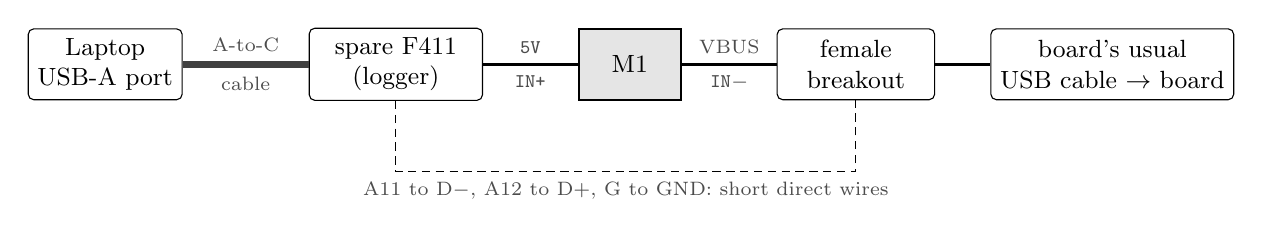
\begin{tikzpicture}[node distance=5mm and 7mm]
\node[blk, minimum width=13mm] (lap) {Laptop\\USB-A port};
\node[blk, right=16mm of lap, minimum width=22mm] (male) {spare F411\\(logger)};
\node[ina, right=12mm of male] (m1) {M1};
\node[blk, right=12mm of m1, minimum width=20mm] (fem) {female\\breakout};
\node[blk, right=of fem, minimum width=24mm] (brd) {board's usual\\USB cable $\to$ board};
\draw[line width=2.4pt, black!75] (lap) -- node[lbl, above] {A-to-C} node[lbl, below] {cable} (male);
\draw[pw] (male) -- node[lbl, above] {\code{5V}} node[lbl, below] {\code{IN+}} (m1);
\draw[pw] (m1) -- node[lbl, above] {VBUS} node[lbl, below] {\code{IN$-$}} (fem);
\draw[pw] (fem) -- (brd);
\draw[dat] (male.south) -- ++(0,-0.9) -| node[lbl, pos=0.25, below] {A11 to D$-$, A12 to D+, G to GND: short direct wires} (fem.south);
\end{tikzpicture}
\caption{Only the 5\,V line goes through M1. The spare F411's \code{5V} pin sits after its input
diode, so the measured board receives about 4.7\,V; M1 records the actual voltage.}
\end{figure}

\textbf{Check first:} with only the spare F411 plugged in and running the logger, \code{dmesg -w}
must print nothing. An \code{error -71} line, or a new device in \code{lsusb}, means something
sits on the data lines (a pull-up, or an image with USB in it) and the arrangement must not be
used until it is gone. Then stream one utterance through the chain and confirm the output is
bit-exact: the data wires are unshielded, so twist them and keep them short.

\textbf{M1 is the blue INA226 module with one 8-pin header} (\code{IN+ IN- VBS ALE SCL SDA GND
VCC}, pins pointing down) and no screw terminal, so the 5\,V goes in and out through its
\code{IN+} and \code{IN-} header pins. \code{VCC}, \code{SCL}, \code{SDA}, \code{GND} go to the
logger (its \code{GND} from the \code{GND} pin of the spare F411's 4-pin end header). \code{ALE}
stays free. \code{VBS} (the bus-voltage sense, no current) cannot share the \code{IN-} pin, so it
goes to the spare F411's \emph{other} 5\,V pin, at the USB end next to \code{G}: the module then
reads the supply side of the shunt, and the logger reports the board's voltage as
$V_\text{bus} - V_\text{shunt}$, exactly the \code{IN-} side, from the two registers it reads
anyway.

\textbf{On the S3, use only the port marked \code{USB}} (the one that carries the audio stream)
and leave \code{COM} unplugged, or part of the board's current comes in through the second
cable and M1 does not see it. The S3 is flashed over \code{COM}, so a new image means plugging
\code{COM} in, flashing, and unplugging it again.

\section{The debugger stays wired}

The debugger is never unplugged during a measurement campaign. Its \code{TXD} goes to the spare
F411's \code{A3}, its \code{RXD} to \code{A2} and one \code{GND} to a \code{G} pin: that is how the
readings reach the laptop. Its \code{SWDIO}, \code{SWCLK} and other \code{GND} go to the SWD pins of
whichever STM32 is measured, so a script can flash one image after another. Its \code{3V3} and
\code{5V} pins are never connected, as always.
The harness keeps the colours it was delivered with, and they break the usual convention:
3V3 red, SWDIO black, SWCLK yellow, GND green, SWO blue, NRST white, TXD orange, RXD purple,
GND brown, 5V light grey. \textbf{Black is a signal here, not ground}; read the label on the
board, not the colour.

\textbf{What the flash leaves behind.} When OpenOCD connects to an STM32 its target script turns on
debug clocks in \code{DBGMCU\_CR} (on the H7 its own comment says \emph{uses more power}), and
that register is cleared only by a power cycle, not by a reset. A board measured straight after a
flash would therefore not be in the state a deployed board is in. The flash script, after its
usual \code{reset run}, writes 0 to \code{DBGMCU\_CR} (F411 \code{0xE0042004}, H723
\code{0x5C001004}), reads it back, and quits OpenOCD; nothing talks to the debug port while a
reading is taken. The SWD lines of an idle debugger are high-impedance, so they carry no current
into the board.

\textbf{Prove it once per STM32 board} before relying on it: idle power after a scripted flash
must equal idle power after unplugging and replugging the board's cable with the SWD wires off,
within the reading's noise. If it does not, replug the board's cable after every flash, which
clears everything.

\section{\texorpdfstring{Raspberry Pi 5: its own telemetry, nothing wired}{Raspberry Pi 5: its own telemetry, nothing wired}}

\textbf{Decided 2 November 2026.} The Pi 5's power-management chip reports the voltage and the
current of each of its supply rails (\code{vcgencmd pmic\_read\_adc}); the Pi's power is the sum
of voltage times current over those rails. Nothing is bought and no session waits for a part.

\textbf{What it leaves out.} The rails are measured after the chip's converters, so the figure
contains neither the conversion losses nor anything fed straight from the 5\,V input (the USB
ports, the fan). The microcontroller figures are taken at the 5\,V input and do contain their
regulators' losses, so the Pi looks better than it would on the same footing, by roughly the
converters' loss. The paper states this beside every Pi energy figure.

\textbf{How.} Sample once a second from a script pinned to a core the benchmark does not use:
the sampler runs on the machine it measures, so it must stay slow and off the measured core.
Log the fan's PWM setting with every reading, keep HDMI and USB devices unplugged, and check
that \code{vcgencmd get\_throttled} reads \code{0x0} before and after.

\section{Rules for every session}
\begin{enumerate}
\item \code{IN+} towards the supply, \code{IN$-$} towards the board, \code{VBUS} on the
\code{IN$-$} side. The shunt always goes in the 5\,V wire, never in the ground.
\item One common ground: module, board and logger.
\item The debugger stays wired, its \code{3V3} and \code{5V} pins disconnected; OpenOCD is not
running while a reading is taken.
\item Run the exact image whose timing figures are in the results (check its checksum),
with nothing else attached.
\end{enumerate}

\section{Calibration, once, before the first board}
\begin{enumerate}
\item Read each shunt's marking with a magnifier and label the modules M1--M6.
\item \textbf{Zero:} with nothing on \code{IN+}/\code{IN$-$}, log each module for a minute;
subtract that offset from everything later.
\item \textbf{Scale:} put one module at a time in series with a multimeter (10\,A range) and a
5\,W load resistor on a 5\,V supply. Read at about 100, 330 and 690\,mA (47, 15 and
6.8\,$\Omega$). The module's ratio to the meter is its correction factor; all modules share
the same meter, so they share one scale. Record the meter's model.
\item No shunt-size cross-check is needed: every module in use is an \code{R100}, and the Pi
is not measured with a module.
\end{enumerate}

\section{One board's session}
\begin{enumerate}
\item Flash the board's measurement image and confirm its checksum: by script on the two STM32
boards (section~4), over \code{COM} on the S3 and then \code{COM} unplugged, by copy on the Pi.
The logger's bus scan must find \code{0x40} only.
\item For each state, wait two minutes and then average one minute of readings:
\begin{itemize}
\item $P_\text{idle}$: board connected, port open, no audio flowing;
\item $P_\text{active}$: audio streamed unpaced, hops back to back;
\item a short paced run as a check: with the logged duty cycle $d$, the reading must equal
$d\,P_\text{active} + (1-d)\,P_\text{idle}$.
\end{itemize}
\item Record the module number, the calibration table version, the cable, the room
temperature and, on the Pi, the fan setting. Unplug everything and move to the next board.
\end{enumerate}

Energy per second of audio is then
$E = P_\text{active}\cdot\text{RTF} + P_\text{idle}\cdot(1-\text{RTF})$, or
$P_\text{active}\cdot\text{RTF}$ when RTF $> 1$. Expect a large idle term on the two STM32
boards (their main loop polls USB at full clock and never sleeps) and a small one on the S3
and the Pi (both wait for an interrupt or a deadline).

\textbf{Check before you start:} the shunt marking on each module (\code{R100}).

\end{document}
